% Paquets généraux
\documentclass[a4paper,12pt,titlepage]{article}
\usepackage[T1]{fontenc}
\usepackage[utf8]{inputenc}
\usepackage[french]{babel}
\usepackage[gen]{eurosym}
%\usepackage[dvips]{graphicx}
\usepackage{fancyhdr}
\usepackage{pdfpages} 
\usepackage{multido}
\usepackage{moreverb}
\usepackage{hyperref}
%\usepackage{textcomp}
\usepackage{verbatim}
\usepackage{moreverb}
\usepackage{listings}
\usepackage{minted}
\usepackage{eso-pic}
\usepackage{enumitem}
\usepackage{comment}
\usepackage{boxedminipage}
\usepackage[french,onelanguage, boxruled,linesnumbered]{algorithm2e}


\newcommand{\auteurun}{Juliette Genzmer}
\newcommand{\auteurdeux}{Willie Robert}
\newcommand{\auteurtrois}{Renaud Costadoat}
\newcommand{\institute}{Lycée Dorian}
\newtheorem{solution}{Solution}


\newcommand{\nom}{Porte conteneur}
\newcommand{\sequence}{03}
\newcommand{\num}{04}
\newcommand{\type}{TD}
\newcommand{\descrip}{Résolution d'un problème en utilisant des méthodes algorithmiques}
\newcommand{\competences}{Alt-C3: Concevoir un algorithme répondant à un problème précisément posé}

\usepackage{color}
\usepackage{xcolor}
\usepackage{colortbl}
\usepackage{helvet}
\renewcommand{\familydefault}{\sfdefault}
\usepackage{amsfonts}
\usepackage{amsmath}
%\usepackage{xspace}
\usepackage{varioref}
\usepackage{tabularx}
%\usepackage{floatflt}
\usepackage{graphics}
\usepackage{wrapfig}
\usepackage{textcomp}
\usepackage{tikz}
\usepackage{wrapfig}
\usepackage{gensymb}
\usepackage{ifthen}
\usepackage{cancel}
\usepackage{etoolbox}
\usepackage{multirow}
%\usepackage{boxedminipage}
\definecolor{gris25}{gray}{0.75}
\definecolor{bleu}{RGB}{18,33,98}
\definecolor{bleuf}{RGB}{42,94,171}
\definecolor{bleuc}{RGB}{231,239,247}
\definecolor{rougef}{RGB}{185,18,27}
\definecolor{rougec}{RGB}{255,188,204}%255,230,231
\definecolor{vertf}{RGB}{103,126,82}
\definecolor{vertc}{RGB}{220,255,191}
\definecolor{forestgreen}{rgb}{0.13,0.54,0.13}
\definecolor{blcr}{rgb}{0.59,0.69,0.84}
\definecolor{blfr}{rgb}{0.32,0.51,0.75}
\definecolor{orfr}{rgb}{0.90,0.42,0.15}
\definecolor{orcr}{rgb}{0.90,0.65,0.50}
\definecolor{orangef}{rgb}{0.659,0.269,0.072}
\definecolor{orange}{rgb}{0.58,0.35,0.063}
\definecolor{orangec}{rgb}{0.43,0.32,0.25}
\definecolor{rcorrect}{rgb}{0.6,0,0}
\definecolor{sequence}{rgb}{0.75,0.75,0.75}
\definecolor{competences}{rgb}{0.61,0.73,0.35}
\definecolor{grisf}{HTML}{222222}
\definecolor{grisc}{HTML}{636363}
\definecolor{normal}{HTML}{4087c4}
\definecolor{info}{HTML}{5bc0de}
\definecolor{success}{RGB}{92,184,92}
\definecolor{warning}{RGB}{240,173,78}
\definecolor{danger}{RGB}{217,83,79}
\hypersetup{                    % parametrage des hyperliens
    colorlinks=true,                % colorise les liens
    breaklinks=true,                % permet les retours à la ligne pour les liens trop longs
    urlcolor= blfr,                 % couleur des hyperliens
    linkcolor= orange,                % couleur des liens internes aux documents (index, figures, tableaux, equations,...)
    citecolor= forestgreen                % couleur des liens vers les references bibliographiques
    }

% Mise en page
\pagestyle{fancy}

\setlength{\hoffset}{-18pt}

\setlength{\oddsidemargin}{0pt} 	% Marge gauche sur pages impaires
\setlength{\evensidemargin}{0pt} 	% Marge gauche sur pages paires
\setlength{\marginparwidth}{00pt} 	% Largeur de note dans la marge
\setlength{\headwidth}{481pt} 	 	% Largeur de la zone de tête (17cm)
\setlength{\textwidth}{481pt} 	 	% Largeur de la zone de texte (17cm)
\setlength{\voffset}{-18pt} 		% Bon pour DOS
\setlength{\marginparsep}{7pt}	 	% Séparation de la marge
\setlength{\topmargin}{-30pt} 		% Pas de marge en haut
\setlength{\headheight}{55pt} 		% Haut de page
\setlength{\headsep}{20pt} 		% Entre le haut de page et le texte
\setlength{\footskip}{30pt} 		% Bas de page + séparation
\setlength{\textheight}{700pt} 		% Hauteur de l'icone zone de texte (25cm)
\setlength\fboxrule{1 pt}
\renewcommand{\baselinestretch}{1}
\setcounter{tocdepth}{1}
\newcommand{\cadre}[2]
{\fbox{
  \begin{minipage}{#1\linewidth}
   \begin{center}
    #2\\
   \end{center}
  \end{minipage}
 }
}

\newcounter{num_quest} \setcounter{num_quest}{0}
\newcounter{num_rep} \setcounter{num_rep}{0}
\newcounter{num_cor} \setcounter{num_cor}{0}

\newcommand{\question}[1]{\refstepcounter{num_quest}\par
~\ \\ \parbox[t][][t]{0.15\linewidth}{\textbf{Question \arabic{num_quest}}}\parbox[t][][t]{0.85\linewidth}{#1\label{q\the\value{num_quest}}}\par\par
}



\newcommand{\reponse}[0]{\refstepcounter{num_rep}\par
~\ \\ \parbox[t][][t]{0.15\linewidth}{\textbf{Question \arabic{num_rep}}}}

\newcommand{\cor}
{\refstepcounter{num_cor}
\noindent
\rule{\linewidth}{.5pt}
\textbf{Question \arabic{num_cor}:} \\
}



% En tête et pied de page
\lhead{\nom}
\rhead{
\includegraphics[width=2cm]{../../../img/logo}}
\lfoot{David Aubert, Renaud Costadoat}
\rfoot{Page \thepage}
\cfoot{}

\newlength{\RoundedBoxWidth}
\newsavebox{\GrayRoundedBox}
\newenvironment{GrayBox}[1][\dimexpr\textwidth-4.5ex]%
   {\setlength{\RoundedBoxWidth}{\dimexpr#1}
    \begin{lrbox}{\GrayRoundedBox}
       \begin{minipage}{\RoundedBoxWidth}}%
   {   \end{minipage}
    \end{lrbox}
    \begin{center}
    \begin{tikzpicture}%
       \draw node[draw=bleuf,fill=bleuc,rounded corners,%
             inner sep=2ex,text width=\RoundedBoxWidth]%
             {\usebox{\GrayRoundedBox}};
    \end{tikzpicture}
    \end{center}}

\fancypagestyle{correction}{%
  \fancyhf{}
  \lhead{\colorbox{danger}{\begin{minipage}{0.65\paperwidth} \textcolor{white}{\textbf{Correction}} \end{minipage}} }
  \rhead{
\includegraphics[width=2cm]{../../../img/logo}}
  \lfoot{Juliette Genzmer, Willie Robert, Renaud Costadoat}
  \rfoot{\colorbox{danger}{\begin{minipage}{0.3\paperwidth} \begin{flushright}\textcolor{white}{\textbf{Correction}}\end{flushright} \end{minipage}} }}

\renewcommand{\footrulewidth}{0.4pt}


\newcommand{\BackgroundPic}{%
\put(0,0){%
\parbox[b][\paperheight]{\paperwidth}{%
\vfill
\begin{center}
\hspace{0.5cm}\vspace{0.5cm}

\includegraphics[width=\paperwidth,height=\paperheight,%
keepaspectratio]{../../../img/fond5}%
\end{center}
\vfill
}}}

\newcommand{\goforum}{
\begin{figure}[ht!]
\begin{center}
 
\includegraphics[width=0.7\linewidth]{../../../img/go_forum}
\end{center}
\label{go_forum}
\caption{J'pète les plombs}
\end{figure}}

\newcommand{\BackgroundPicdeux}{%
\put(25,-30){%
\parbox[b][\paperheight]{\paperwidth}{%
\vfill
\begin{center}

\includegraphics[width=\paperwidth,height=\paperheight,%
keepaspectratio]{../../../img/fond6}%
\end{center}
\vfill
}}}

\setenumerate[1]{align=left,label=\arabic*}
\setenumerate[2]{before=\stepcounter{enumi},label*=.\arabic*,leftmargin=1.2em,align=left}

\begin{document}


\pagestyle{fancy}

\AddToShipoutPicture{\BackgroundPicdeux}

\begin{center}
{\Large\bf {\type} \no {\numero} -- \descrip}
\end{center}

\SetKw{KwFrom}{de} 

\begin{boxedminipage}{.9\textwidth} 
\begin{itemize}
 \item Faire tous les exercices dans un fichier {NomPrenom.py} à sauvegarder,
 \item mettre en commentaire l'exercice et la question traités (ex: \# Exercice 1),
 \item ne pas oublier pas de commenter ce qui est fait dans votre code (ex: \# Je crée une fonction pour calculer la racine d'un nombre),
 \item il est possible de demander un déblocage pour une question, mais celle-ci sera notée 0,
 \item il faut vérifier avant de partir que le code peut s'exécuter et qu'il affiche les résultats que vous attendez. Les lignes de code qui doivent s'exécuter sont décommentées.
\end{itemize}
\end{boxedminipage}

\section{Coupe du monde de rugby}

\begin{minipage}{0.6\linewidth}
Le classement des poules s'effectue en comptant le nombre de points de chaque équipe.\\ Une victoire (V) rapporte 4 points, un match nul (N) (égalité) 2 points et une défaite (D) 0 point et à ses points s'ajoutent des points de bonus (BP).\\
Ainsi la France possède pour le moment $3\cdot 4+0\cdot 2+1=13$ points.
\end{minipage}\hfill
\begin{minipage}{0.35\linewidth}
\centering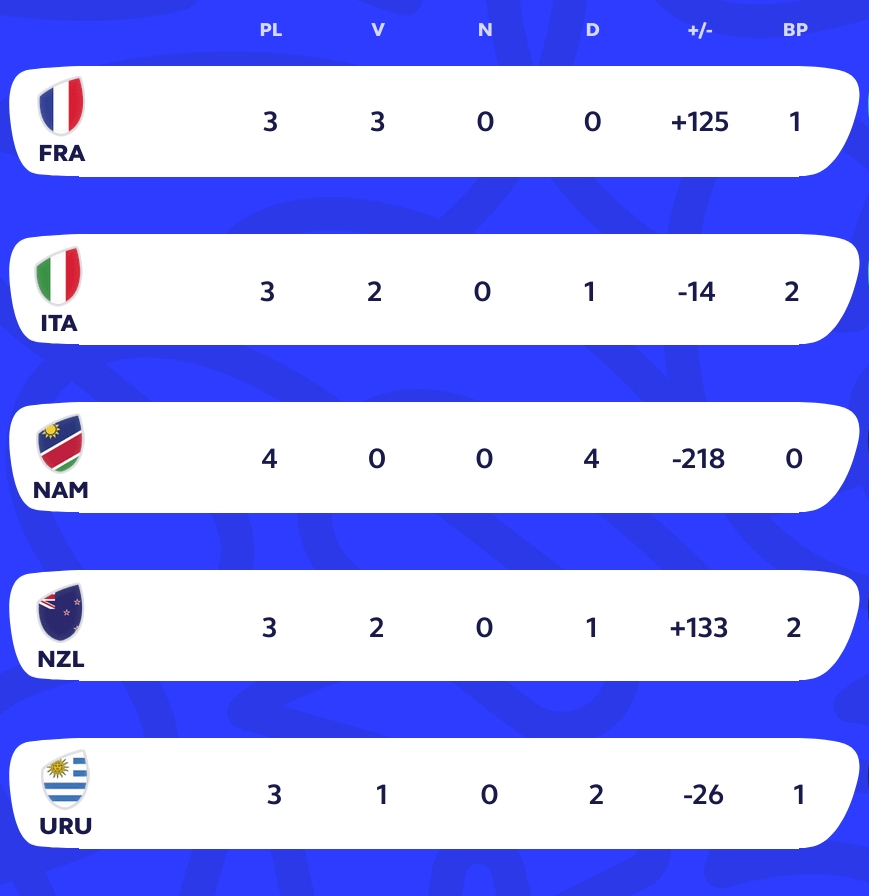
\includegraphics[width=0.7\linewidth]{img/groupe_A}
\end{minipage}

\vspace{0.5cm}

Le script python ci-dessous permet d'établir le classement mais il doit être complété.

Il est disponible dans le dossier \og \texttt{/home/eleve/Ressources/PTSI/script\_rugby.py}\fg, vous pouvez copier/coller son contenu dans votre script.

\begin{minted}[linenos]{python}
colonnes=['Nom pays','Victoires','Nuls','Défaites','Differences points',\
'Points bonus','Total points']
groupe_A=[['France',3,0,0,125,1,0],['Italie',2,0,1,-14,2,0],\
['Namibie',0,0,4,-218,0,0],['Nouvelle-Zélande',2,0,1,133,2,0],\
['Urugay',1,0,2,-26,1,0]]

def calcul_points(equipe):
    return equipe[1]+equipe[2]

for equipe in groupe_A:
    equipe[...]=calcul_points(equipe)

def sort_key(equipe):
    return equipe[6],equipe[4]

groupe_A.sort(key=sort_key, reverse=True)

for equipe in groupe_A:
    print(equipe)
\end{minted}

\newpage

\question{\textbf{Modifier} la fonction \texttt{calcul\_points} aux lignes 7 et 8 afin qu'elle utilise les critères propres à la compétition afin d'établir les scores. Tester le résultat en affichant \texttt{print(calcul\_points(['France',3,0,0,125,1,0]))}.}

\question{\textbf{Modifier} la ligne 11 afin que le script enregistre les scores à la suite des données de chaque équipe. Ainsi, la liste liée à la France devient \texttt{['France', 3, 0, 0, 125, 1, 13]}.}

\section{La légende de Sissa}

La légende de Sissa est un mythe qui raconte l'invention du Chaturanga, la forme indienne du jeu d'échecs.

Le brahmane ou sage Sissa (ou Sessa) Sissa Ibn Dahir est un personnage mythique de l'Inde. 

En Inde, le roi Belkib (ou Bathait), qui s'ennuie à la cour, demande qu'on lui invente un jeu pour le distraire. Le sage Sissa invente alors le Chaturanga, l'ancêtre du jeu d'échecs, ce qui ravit le roi. Pour remercier Sissa, le roi lui demande de choisir sa récompense, aussi fastueuse qu'elle puisse être. Sissa choisit de demander au roi de prendre le plateau du jeu et, sur la première case, poser un grain de riz, ensuite deux sur la deuxième, puis quatre sur la troisième, et ainsi de suite, jusqu'à la 64ème, en doublant à chaque fois le nombre de grains de riz que l’on met.

Le roi et la cour sont amusés par la modestie de cette demande. Le roi tente de persuader Sissa d'accepter une récompense d'une valeur plus importante. Devant le refus de Sissa, il ordonne que les grains soient apportés. Mais lorsqu'on met en \oe uvre la demande, on s'aperçoit qu'il n'y a pas assez de grains de riz dans tout le royaume pour la satisfaire. 

~\

Extrait de la page Wikipédia \og \texttt{https://fr.wikipedia.org/wiki/Légende\_de\_Sissa} \fg.

~\

La résolution du problème de l'échiquier de Sissa est un exercice algorithmique consistant à déterminer le nombre de grains de riz que devrait obtenir Sissa.

\question{\textbf{Coder} la résolution de ce problème et \textbf{afficher} le nombre de grains de riz que demande Sissa.}

~\

Le poids d'un grain de riz est d'environ 28g.

\question{\textbf{Calculer}, à l'aide de python à la suite de votre script, la masse (en tonnes) des grains de riz dus à Sissa.}

\section{Propriété des multiples de 3}

Un nombre entier est divisible par 3 quand la somme de ses chiffres est un multiple de 3 et uniquement dans ce cas.

ex:
\begin{itemize}
 \item 7 152 est divisible par 3 car 7+1+5+2=15 et 15 est un multiple de 3,
 \item 835 n'est pas divisible par 3 car 8+3+5=16 n'est pas divisible par 3.
\end{itemize}

Dans le but de chercher un contre exemple, on va vérifier cette propriété pour les 1000 premiers entiers.

En sachant que :
\begin{itemize}
 \item \texttt{nombre//10} renvoi le quotient de la division euclidienne de \texttt{nombre} par \texttt{10},
 \item \texttt{nombre\%10} renvoi le reste de la division euclidienne de \texttt{nombre} par \texttt{10},
 \item \texttt{a==b} renvoie \texttt{True} si $a=b$ et 0 si ce n'est pas le cas,
 \item \texttt{a!=b} renvoie \texttt{True} si $a\neq b$ et 0 si ce n'est pas le cas.
\end{itemize}

L'algorithme suivant permet de coder la fonction \texttt{somme\_chiffres} qui permet de sommer tous les chiffres d'un nombre:

~\

\begin{minipage}{0.45\linewidth}
\begin{enumerate}
 \item Mise à 0 de \texttt{somme},
 \item Tant que le quotient de la division de \texttt{nombre} par 10 est positif:
 \begin{enumerate}
  \item \texttt{reste} est le reste de la division euclidienne de \texttt{nombre} par 10,
  \item \texttt{nombre} est le quotient de la division euclidienne de \texttt{nombre} par 10,
  \item ajouter \texttt{reste} à \texttt{somme}
 \end{enumerate}
 \item ajouter \texttt{nombre} à \texttt{somme}
 \item retourner \texttt{somme}.
\end{enumerate}
\end{minipage}\hfill
\begin{minipage}{0.45\linewidth}
Exemple : soit le \texttt{nombre} 1234.

\begin{center}
\begin{tabularx}{200pt}{|X|X|X|}
\hline
nombre & reste & somme \\
\hline
1234 & 0 & 0 \\
\hline
123 & 4 & 4 \\
\hline
12 & 3 & 7 \\
\hline
1 & 2 & 9 \\
\hline
0 & 1 & 10 \\
\hline
\end{tabularx}
\end{center}

Le résultat est 10, et en effet, 1+2+3+4=10.
\end{minipage}

~\

\question{\textbf{Coder} la fonction \texttt{somme\_chiffres(nombre)} qui renvoie la somme des chiffres de nombre. La tester sur le nombre 1234.}

~\

Le code suivant utilise la fonction déterminée à la question précédente, il renvoie 'Faux' si l'hypothèse précédente n'est pas validée (en théorie, cela ne doit jamais arriver.)

\begin{minted}[linenos]{python}
for i in range(1,10**4):
    if somme_chiffres(i).......: # si la somme des chiffres est un multiple de 3
        if ......:  # si le nombre n'est pas un multiple de 3
            print('Faux')
    else:
        if ......: si le nombre est un multiple de 3
            print('Faux')
\end{minted}

\question{\textbf{Compléter} le code précédent afin de vérifier l'hypothèse pour les entiers de 1 à 9999.}

~\

Afin de tester si le résultat de la somme des chiffres est divisible par 3, on souhaite remplacer le test de la ligne 2 par un test qui consisterait à déterminer la somme des chiffres de ce résultats jusqu'à ce que celui-ci soit ramené à un seul chiffre : 3, 6 ou 9.

Exemple : \texttt{somme\_chiffres(9384)=24} or \texttt{somme\_chiffres(24)=6} donc divisible par 3.

\question{\textbf{Proposer} une nouvelle version du code précédent incluant cette nouvelle solution.}


\begin{center}
\Large{FIN}
\end{center}

\cleardoublepage

\ifdef{\public}{\end{document}}{\pagestyle{correction}}


\begin{center}
\Large{Correction}
\end{center}

\reponse{}

\begin{minted}{python}
def calcul_points(equipe):
    return equipe[1]*4+equipe[2]*2+equipe[5]
print(calcul_points(['France',3,0,0,125,1,0]))
\end{minted}

\reponse{}
\begin{minted}{python}
for equipe in groupe_A:
    equipe[6]=calcul_points(equipe)
\end{minted}

\reponse{}

\begin{minted}{python}
somme=0
for i in range(64):
    somme+=2**i

print(somme)
\end{minted}

\reponse{}

\begin{minted}{python}
poids=0.028

total=somme*poids
print(total/1000)
\end{minted}

\reponse{}

\begin{minted}{python}
def somme_chiffres(nombre):
    somme=0
    while nombre//10>0:
        reste=nombre%10
        nombre=nombre//10
        somme+=reste
    somme+=nombre
    return somme
\end{minted}


\reponse{}

\begin{minted}{python}
for i in range(10**4):
    if somme_chiffres(i)%3==0:
        if i%3!=0:
            print('Faux')
    else:
        if i%3==0:
            print('Faux')
\end{minted}

\end{document}